\chapter{Results}
\label{ch:results}
In this chapter we show the results from our experiments. From running all the experiments we got a lot of raw data. This data alongside all the programs tested are on a publicly available git repository. On that git repository you can also find the programs used to do the measurements, the calculations of various statistical tests and all the intermediate results. The link to this repository is \url{https://github.com/lukaskoedijk/Green-Software}. The ordering of the chapter will be as followed, where we first take a loot at the anomaly detection that was done. Secondly we show the results from the experiments concerning the programming languages. After that we will show the results of the experiments when looking at programs. Finally some additional results are shown.

% In this chapter, we present the results of our experiment. 

% table with languages
% table with programs averages
% figure per problem
% example figure of a problem with different programs in same language
% anomalies
% same distribution

% without flags, takes more energy

% For binarytrees: php cosumes the most, python ruby and csharp also relatively bad 
% For fannkuchredux: php python ruby really bad, javascript also not so good
% For fasta: php python ruby javascript not good
% For mandelbrot: python php ruby not good
% For nbody: python php ruby not good
% For revcomp: not one that really stands out, though c++-noflags has a huge range thus potentially really bad
% For spectralnorm: python least good, php ruby also not good

% Overall php, python and ruby not good conform the energy consumption

\section{Anomalies}
We checked for anomalies using DBSCAN. An example of the results we got from this approach is shown in figure \ref{fig:anomalies}. There we can see in the top graph the distribution of measurements for a single program on one of the two nodes on the DAS. The red dots are the measurements DBSCAN labelled as an anomaly. In the bottom graph we see from every measurement point its distance to its fourth nearest neighbour. This is sorted and the red dot is the choice of the input variable of DBSCAN called \textit{eps} and is calculated by finding the first valley.\\

For \textit{node28} there were a total of 345 anomalies from 7263 measurement points, which is roughly 4.8\%. In the measurements from \textit{node29} there were a total of 305 anomalies from 5918 measurement points found, which is roughly 5.1\%. Even though there are more anomalies found than programs, there was not for every program an anomaly detected. All the anomalies found were removed from further results.

\begin{figure}[h]
    \centering
    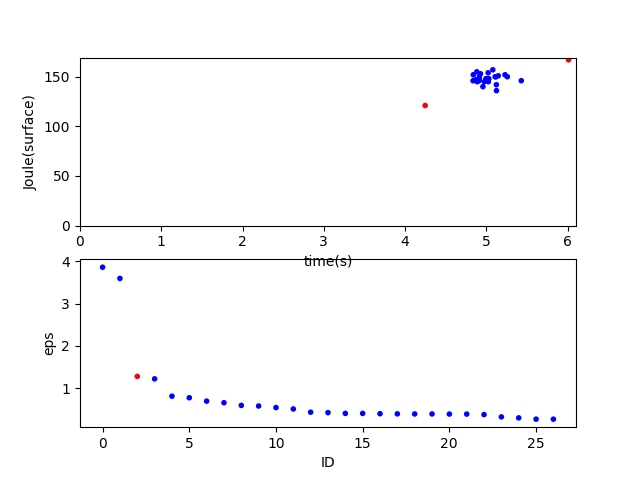
\includegraphics[width=.6\textwidth]{graphs/port3-bdscan-java-3-problem0-eps1-27.png}
    \caption{In the top graph the distribution of measurements from program java-3 on the Binarytrees problem on \textit{node28} is shown. The bottom graph shows the sorted fourth nearest neighbour graph. The red dots at the top are measurements labelled as an anomaly and at the bottom is the choice for the \textit{eps}-value.}
    \label{fig:anomalies}
\end{figure}

\subsection{Two clusters}
During the processing of the information from the anomaly detection we saw only on \textit{node29} that the resulting measurements for some programs could be clustered. We looked further into this and found that where we found two clusters it seemed to follow an ordering based on the moment of measuring. With clusters based on the moment of measuring we mean that in the first cluster all measurements were done before a certain date and in the second cluster after that date. The DBSCAN algorithm found for \textit{node28} seven times two clusters in the measurements for a single program, none of which follow the moment of measuring, and 58 times for \textit{node29} of which 53 follow the moment of measuring. At \textit{node29} for all of these 53 programs the null hypothesis that they're from the same distribution can be rejected. We then instead of letting a clustering algorithm cluster first and then check if the clusters follow the moment of measuring, clustered ourselves based on the moment of measuring. We find that for \textit{node28} 218 programs and for \textit{node29} 41 programs the null hypothesis that the two moment of measuring clusters are from the same population can't be rejected. Because of the large amount of programs where the clusters were not from the same population at \textit{node29}, we decided to run another clustering algorithm named k-means. We set the amount of clusters the k-means algorithm will search for at two, because we wanted to find these two moment of measuring clusters. We then found that there were zero programs that had clusters based on moment of measuring for \textit{node28} and 63 programs for \textit{node29}. These 63 programs all rejected the null hypothesis that the two clusters were from the same population. When looking at the programming languages and problems these 63 programs entail, we saw a good representation of the programming languages and different problems. There were no indications of suspecting some programming language or problem specific cause for this difference. There still could be some other commonality between these programs, but it is too difficult to find this between the 63 programs. Therefor we left it like this with on \textit{node28} no difference in the moment of measuring and on \textit{node29} only a difference in some of the programs.
%Therefor this is where we left it with on \textit{node28} no difference in the moment of measuring and on \textit{node29} only a difference in a part of the programs.

\section{Programming Languages}
After all the measurements were done we wanted to compare the programming languages. This was done by filtering out one problem and selecting every measurement of a program that solves this problem. This resulted in a lot of points per language and these are plotted in a box-plot. There are seven problems and thus also seven box-plots. An example of one of these box-plots is shown in figure \ref{fig:box-example}. Here the box is from the first quartile till the third quartile and a line at the median. The dots are measurement points laying outside the fences that are located at $Q1 - 1.5(Q3-Q1)$ and $Q3 + 1.5(Q3-Q1)$. The whiskers show the range of points that are outside the box but inside the fences. All the graphs are shown in appendix \ref{app:node28} for \textit{node28} and appendix \ref{app:node29} for \textit{node29}.\\

\begin{figure}[h]
    \centering
    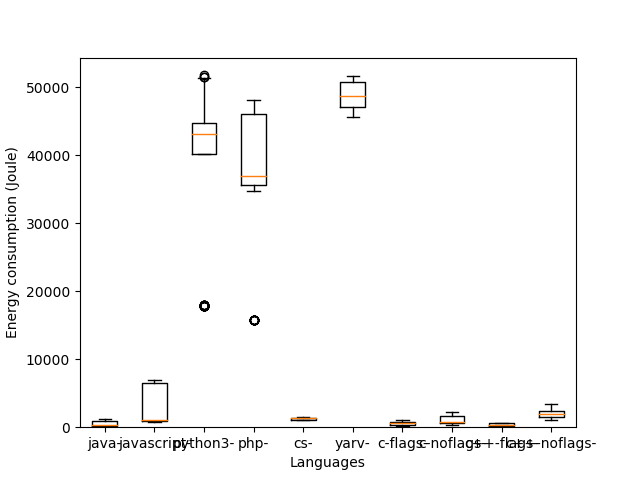
\includegraphics[width=.6\textwidth]{graphs/fannkuchredux_BOXoverview3.png}
    \caption{The box plot of the different programs in a programming language for the problem Fannkuchredux on \textit{node28}.}
    \label{fig:box-example}
\end{figure}

In the box-plot we can't always clearly see which programming language is using less energy. To find out what the relationship is between two programming languages we used twice the one-sided Mann Whitney U test. This we calculated for every language with every other language and because of the fact that if one is smaller the other should be larger this table should be inverted around the diagonal zero's, thus a \textit{+} changes into a \textit{-}. An example of this is shown in table \ref{tab:lang-example}. In that table a \textit{+} means that the programming language on the row is performing better than the programming language on the column, i.e. the programming language on the row consumes less energy. The \textit{-} means the opposite, a \textit{0} means equal and \textit{unknown} means that both one-sided Mann Whitney U tests could not be rejected. All the tables are shown in appendix \ref{app:node28} for \textit{node28} and appendix \ref{app:node29} for \textit{node29}.\\

\begin{table}[h]
\centering
\resizebox{\textwidth}{!}{%
\begin{tabular}{|l|c|c|c|c|c|c|c|c|c|c|}
\hline
 & \multicolumn{1}{l|}{Java} & \multicolumn{1}{l|}{JavaScript} & \multicolumn{1}{l|}{Python} & \multicolumn{1}{l|}{PHP} & \multicolumn{1}{l|}{C\#} & \multicolumn{1}{l|}{Ruby} & \multicolumn{1}{l|}{C-flags} & \multicolumn{1}{l|}{C-noflags} & \multicolumn{1}{l|}{C++-flags} & \multicolumn{1}{l|}{C++-noflags} \\ \hline
Java& 0 & + & + & + & + & + & - & + & - & +\\ \hline
JavaScript & - & 0 & + & + & + & + & - & + & - & +\\ \hline
Python& - & - & 0 & - & - & - & - & - & - & -\\ \hline
PHP & - & - & + & 0 & - & - & - & - & - & -\\ \hline
C\# & - & - & + & + & 0 & + & - & + & - & +\\ \hline
Ruby & - & - & + & + & - & 0 & - & - & - & -\\ \hline
C-flags & + & + & + & + & + & + & 0 & + & Unknown & +\\ \hline
C-noflags & - & - & + & + & - & + & - & 0 & - & +\\ \hline
C++-flags & + & + & + & + & + & + & Unknown & + & 0 & +\\ \hline
C++-noflags & - & - & + & + & - & + & - & - & - & 0\\ \hline
\end{tabular}%
}
\caption{The comparison of the different languages for the Nbody problem on \textit{node28}. A \textit{+} means that the language on the row has a lower energy consumption then the language on the column, the opposite for \textit{-}, and the \textit{Unknown} means that we could not reject the null hypothesis.}
\label{tab:lang-example}
\end{table}

Using these tables we can see which language is performing better compared to others, but only for a single problem at a time. To give a total overview of problems and programming languages we calculated a score for every combination. One point was rewarded when there was a plus, one point was subtracted when there was a minus and nothing was added or subtracted in the case of a zero or unknown. With the use of these scores we made a heatmap, where green means a high score and red a low. This heatmap is shown in figure \ref{fig:heatmap_L}. Here the programming languages with a lot of green in their row, or a lot of red in their column, are performing better than most programming languages. We also wanted to see which programming language combination resulted the most in an \textit{unknown}, thus which combination could not reject the null hypothesis the most. For this we also created a heatmap where a one was added for every \textit{unknown} found. This resulted in figure \ref{fig:heatmap}.

% Looking at the tables the ordering for the problem Binarytrees is: C++-flags $<$ Java $<$ C-flags $<$ C-noflags $<$ JavaScript $<$ C++-noflags $<$ C\# $<$ Ruby $<$ Python $<$ PHP. \\
% The ordering for Fannkuchredux is: Java $<$ C++-flags $<$ C-flags $<$ C-noflags $<$ JavaScript $<$ C\# $<$ C++-noflags $<$ PHP $<$ Python $<$ Ruby. \\
% The ordering for Fasta is: C-flags $<$ C++-flags $<$ Java $<$ C\# $<$ C-noflags $<$ C++-noflags $<$ JavaScript $<$ PHP $<$ Ruby $<$ Python. \\
% The ordering for Mandelbrot is: (JavaScript = C-flags = C++-flags) $<$ Java $<$ (C\# = C-noflags) $<$ C++-noflags $<$ PHP $<$ (Python = Ruby). \\
% The ordering for Nbody is: (C-flags = C++-flags) $<$ Java $<$ JavaScript $<$ C\# $<$ C-noflags $<$ C++-noflags $<$ Ruby $<$ PHP $<$ Python. \\
% The ordering for Revcomp is: PHP $<$ C-flags $<$ (C-noflags = C++-flags = C\#) $<$ Java $<$ C++-noflags $<$ Python $<$ Ruby $<$ JavaScript. \\
% The ordering for Spectralnorm is: C-flags $<$ C++-flags $<$ (C++-noflags = C\#) $<$ C-noflags $<$ JavaScript $<$ Java $<$ (PHP = Ruby) $<$ Python.\\
% These are the orders for the data from \textit{node28}. The orders for the data form \textit{node29} are almost the same, there are only more languages that are equal concerning the energy consumption.

\begin{figure}[h]
    % \begin{center}
    \begin{subfigure}[b]{0.45\textwidth}
        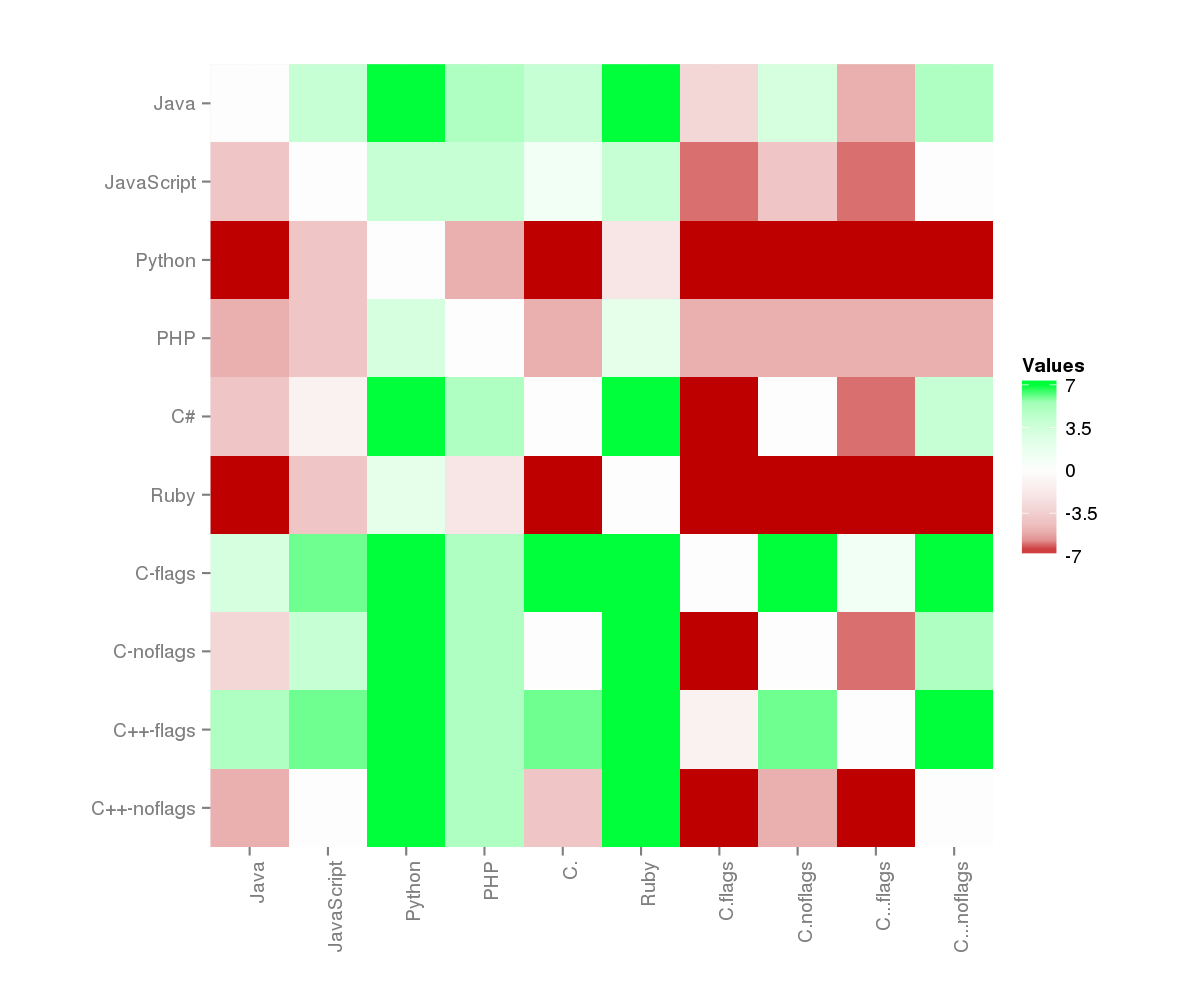
\includegraphics[width=\textwidth, height=6cm]{graphs/heatmapL3.png}
        \caption{The heatmap of \textit{node28} of the relationship between the programming languages for all problems combined. A green box means that the language on the row has a lower energy consumption over all the programs than the language in the column, red is the reverse.}
        \label{fig:heatmap_L3}
    \end{subfigure}
    \hfill        
    \begin{subfigure}[b]{0.45\textwidth}
        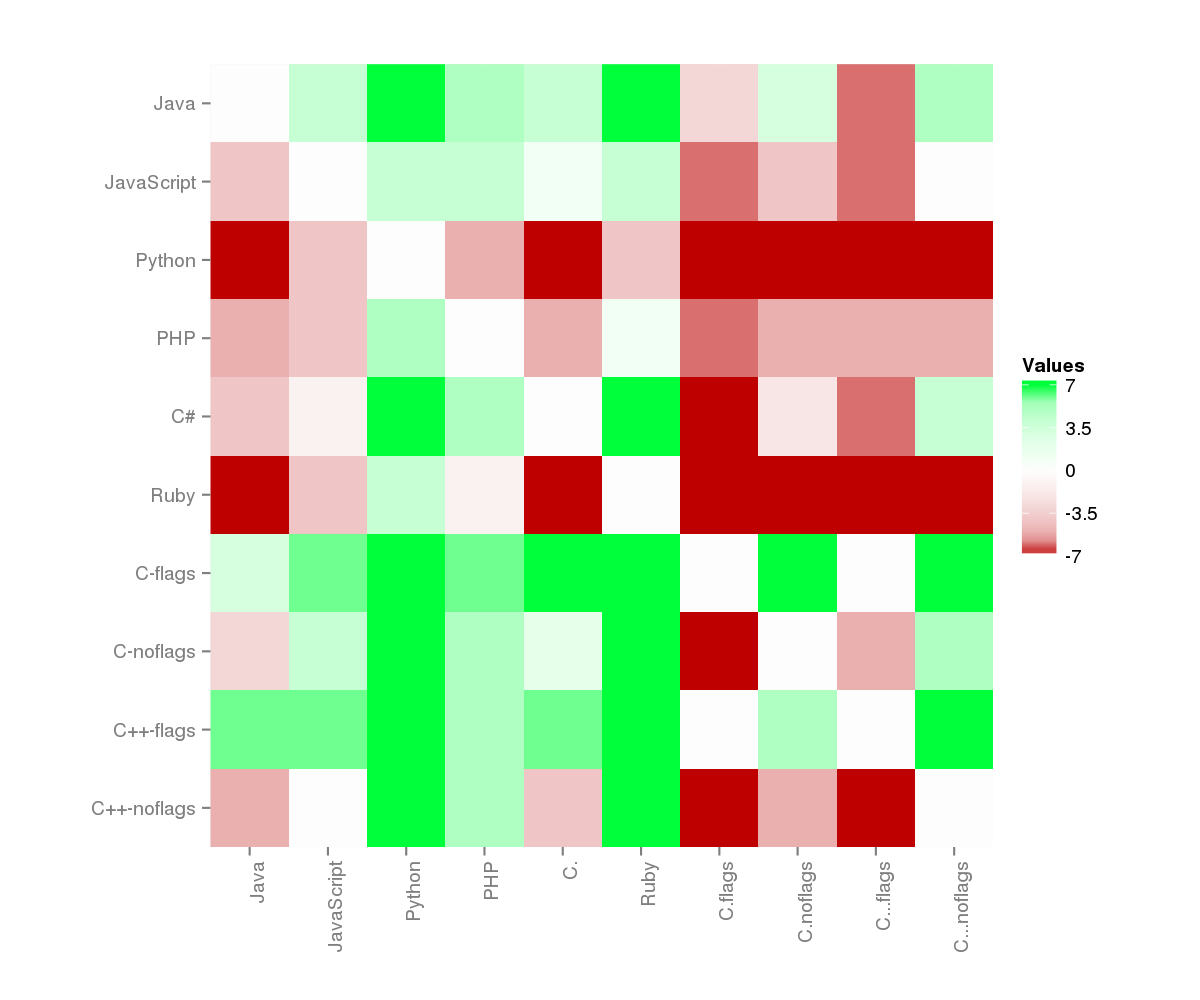
\includegraphics[width=\textwidth, height=6cm]{graphs/heatmapL2.png}
        \caption{The heatmap of \textit{node29} of the relationship between the programming languages for all problems combined. A green box means that the language on the row has a lower energy consumption over all the programs than the language in the column, red is the reverse.}
        \label{fig:heatmap_L2}
    \end{subfigure}
    % \end{center}
    \caption{}
    \label{fig:heatmap_L}
\end{figure}

\begin{figure}[h]
    % \begin{center}
    \begin{subfigure}[b]{0.45\textwidth}
        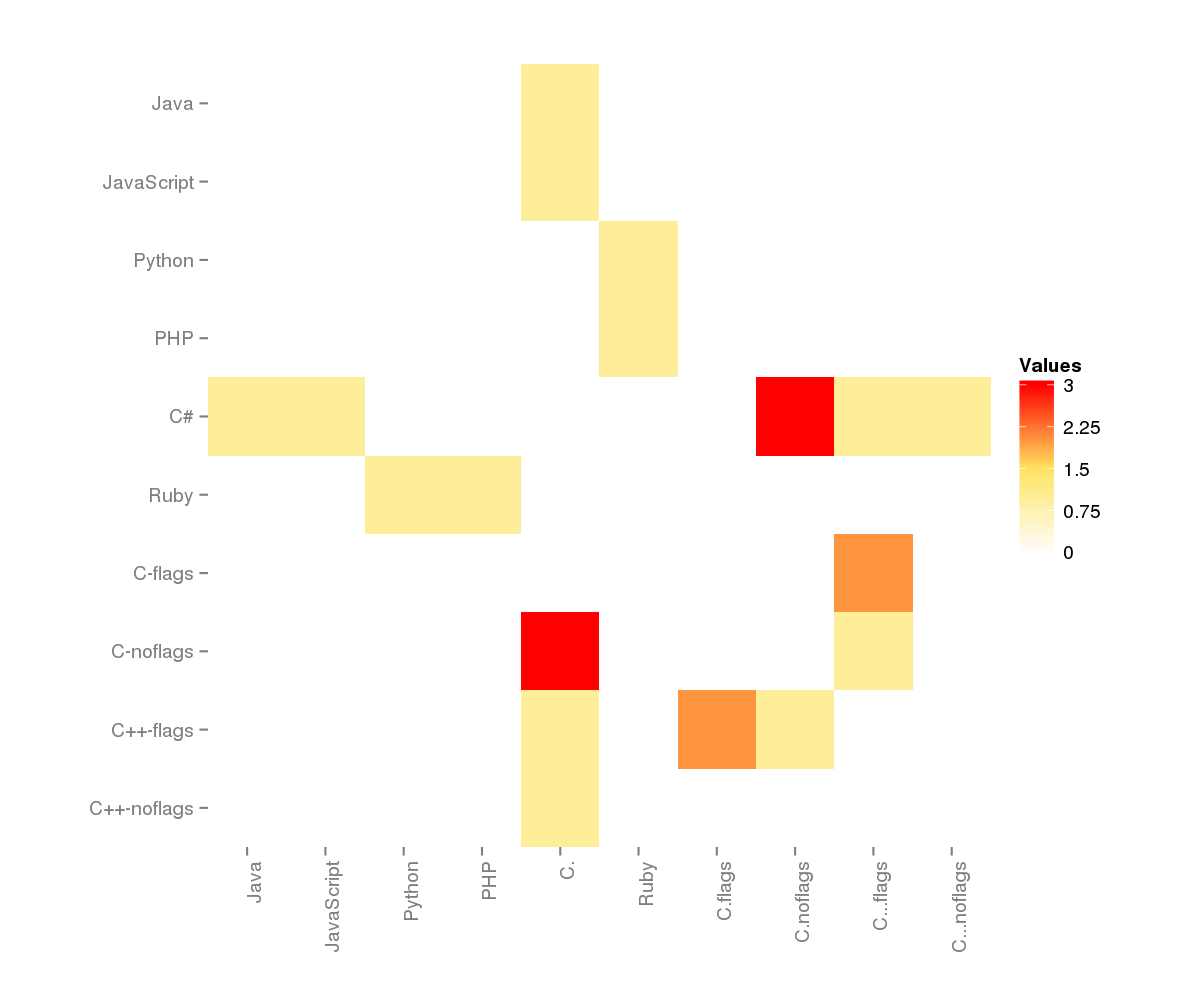
\includegraphics[width=\textwidth, height=6cm]{graphs/heatmap3.png}
        \caption{The heatmap of \textit{node28} of the the amount of times we could not reject the null hypothesis for the relationship between the programming languages for all problems.}
        \label{fig:heatmap_3}
    \end{subfigure}
    \hfill        
    \begin{subfigure}[b]{0.45\textwidth}
        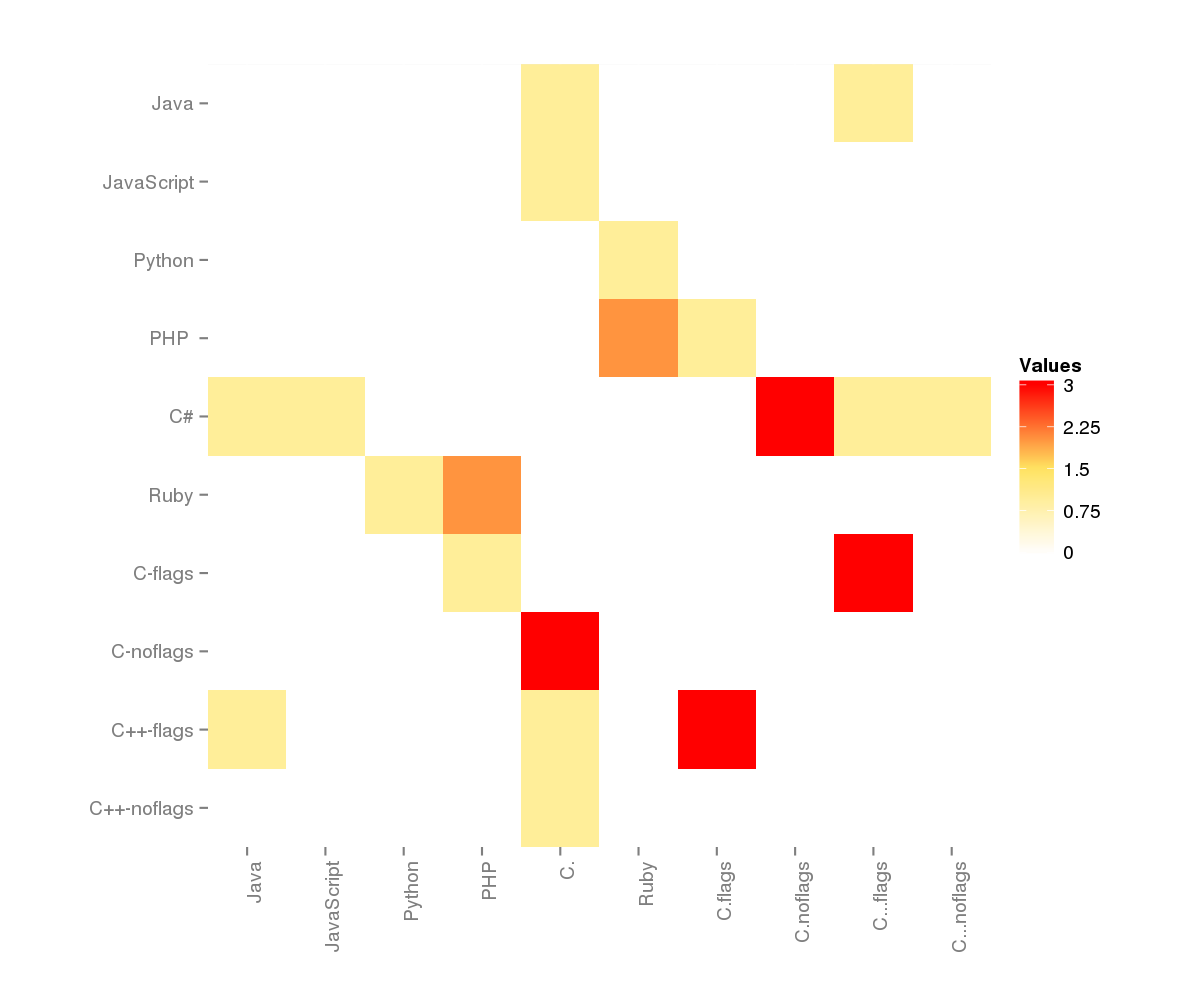
\includegraphics[width=\textwidth, height=6cm]{graphs/heatmap2.png}
        \caption{The heatmap of \textit{node29} of the the amount of times we could not reject the null hypothesis for the relationship between the programming languages for all problems.}
        \label{fig:heatmap_2}
    \end{subfigure}
    % \end{center}
    \caption{}
    \label{fig:heatmap}
\end{figure}

\section{Programs}
When comparing programs that are written in one language and solve the same problem, we can also use a box-plot. An example of such a box plot is shown in figure \ref{fig:box-lang}. Here we can't always see which program is performing better concerning the energy consumption. Therefor we also used the one-sided Mann Whitney U test twice here. For some combination of two programs we weren't able to reject both the Mann Whitney U tests. All these program combinations and their \textit{p}-values are listed in table \ref{tab:programs_equal3} for \textit{node28} and in table \ref{tab:programs_equal2} for \textit{node29} in respectively appendix \ref{app:node28} and \ref{app:node29}. There were a total of 24 program combinations on \textit{node28} and 59 on \textit{node29} where the null hypothesises could not be rejected. We tried to also use Kolmogorov-Smirnov test to see if we would get less cases of uncertainty. This resulted in a total of 33 program combinations for \textit{node28} and 61 for \text{node29}. But when we look at the overlap we see that there are only 24 program combinations for \textit{node28} and 50 for \textit{node29}. Thus this second test removed the uncertainty of nine program combinations on \textit{node29}.

\begin{figure}[h]
    \centering
    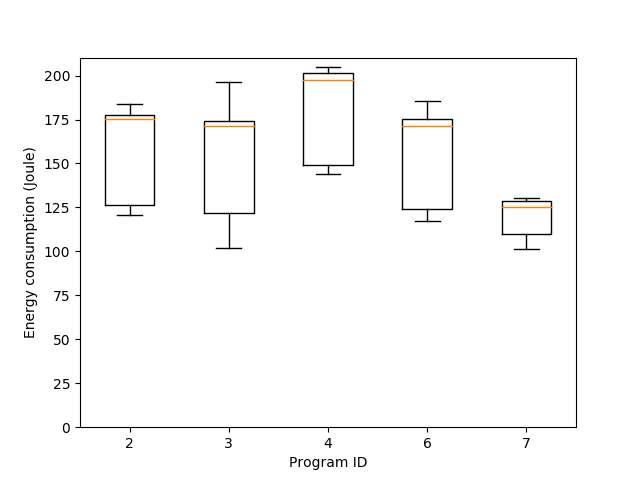
\includegraphics[width=.6\textwidth]{graphs/BOXGroup-java-problem0-3.png}
    \caption{The box-plot for the programming language Java comparing the measurements of different programs that solve the Binarytrees problem and are measured on \textit{node28}.}
    \label{fig:box-lang}
\end{figure}

\subsection{Code level}
When comparing the different programs we found the differences shown in table \ref{tab:code-level} in appendix \ref{app:code-level}. Here we find for most comparisons multiple differences. If there are multiple differences found we can't be sure that a specific difference has an influence on the energy consumption, but if we only see one difference that does not mean that there aren't any other differences. Another problem with multiple differences is that the difference is relative. One way of writing code can be better then a second way of writing code, but worse than a third regards the energy consumption. When looking at table \ref{tab:code-level} we see that multithreading is a lot of times a difference, but it occurs in both the good and bad programs. This can also be said for the difference between a while and for-loop. We also see that using a library instead of implementing it yourself is beneficial concerning the energy consumption.\\

It is really hard to exactly point out what causes the programs to be different, a better approach would be to make a small change in one program when you have two exactly the same programs. To give an example of how this is done we did this for two small changes. The first change we choose was the difference between while and for-loop, because we saw in the table that both occurred in the good and bad section. For the second change we choose the difference between an if-statement with condition and body on different lines and an if-statements with condition and body on the same line, because we expected this to not have an effect. These four programs are shown in \ref{app:code-level}. When we measure the energy consumption 30 times each for these four programs we get the results show in figure \ref{}. Using the Mann Whitney U test we find that there is a significant difference between the \textit{for-loop} program and the \textit{while-loop} program, but we couldn't reject the null hypothesis when comparing the \textit{sameline} and \textit{diffline} programs.

\begin{figure}[h]
    \centering
    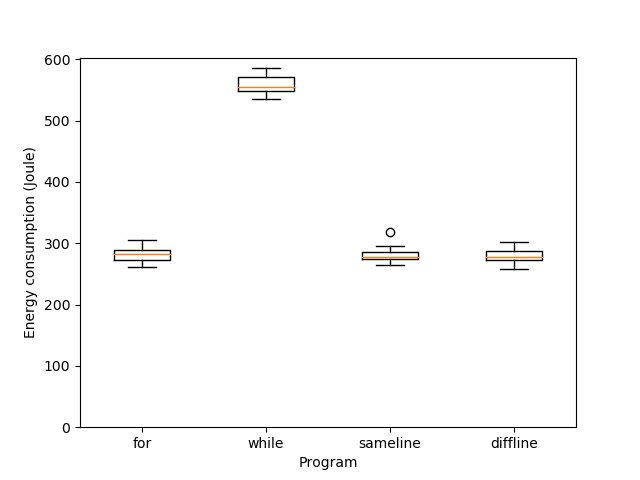
\includegraphics[width=.6\textwidth]{graphs/codelevel.png}
    \caption{The box-plot comparing two programs that have a small difference on code level when solving the 10000th prime number problem. The measurements were done on \textit{node28} and the program were measured 30 times each.}
    \label{fig:box-code}
\end{figure}

% To get a bit of an idea if our finding are correct we made two Python programs, where one according to our findings should perform better conform the energy consumption. Because for different programming languages these difference could be different we only looked at the difference found in Python programs when creating these two programs. The findings we used are that a better programs concerning the energy consumption has the body below the condition in an if-statement, less depth, use library and use while-loop and a worse has body and condition of an if-statement on the same line, more depth, don't use library and use for-loop. 

\section{Additional Findings}
\subsection{Hardware}
Our measurements were run on two different nodes, which had different hardware specifications. To find out how big of an influence the node is we wanted to compare the measurements between the two nodes for a single program. We first used the one-sided Mann Whitney U test and found that for two programs we couldn't reject the null hypothesis that they're from the same distribution. For most programs their energy consumption highly depends on which node they were run on. To see if only the height is different, but still follow the same trend we calculated the correlation. This correlation was calculated between the different programs and an example of the results is shown in figure \ref{fig:corr-example}. In this figure we have positive and negative numbers, this only shows the direction of the correlation. Thus the correlation number $0.7$ and $-0.7$ have the same correlation strength. All the other graphs of the other problems are shown in appendix \ref{app:corr}. In all these graphs we see that most scores are low. Because the distribution of the programs are small we decided to check the correlation of all the measurements in one language for one problem. These are also all listed in appendix \ref{app:corr} and an example is show here in figure \ref{fig:corr-lang-example}. There we see that in most cases the Kendall correlation score is higher.

\begin{figure}[h]
    \begin{subfigure}[b]{0.45\textwidth}
        \centering
        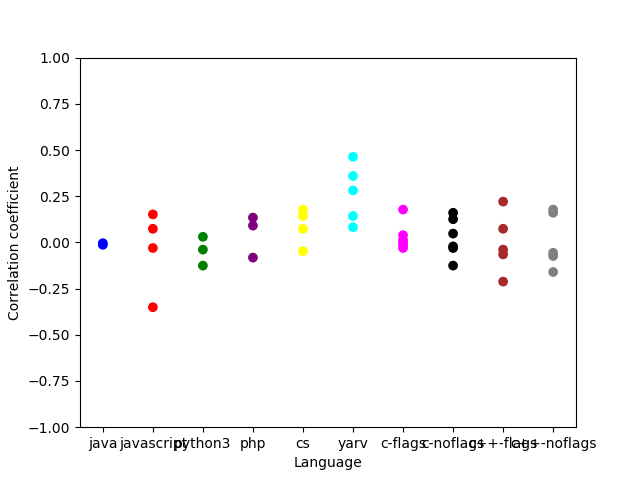
\includegraphics[width=1.1\textwidth]{graphs/kendall_Fasta.png}
        \caption{The Kendall correlation score for every single program that solves the Fasta problem.}
        \label{fig:corr-example}
    \end{subfigure}
    \hfill        
    \begin{subfigure}[b]{0.45\textwidth}
        \centering
        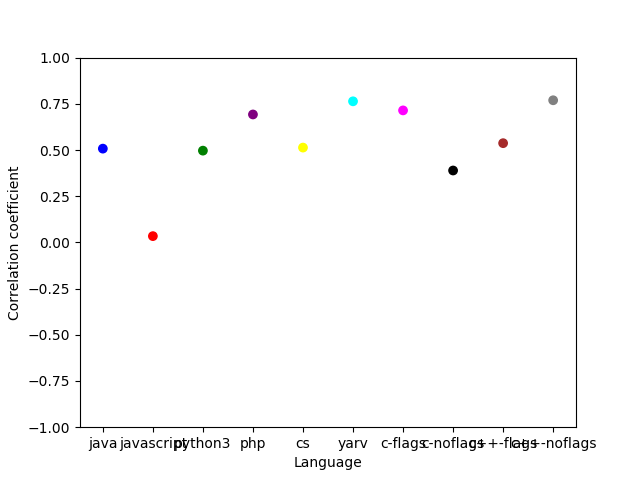
\includegraphics[width=1.1\textwidth]{graphs/kendall-lang_Fasta.png}
        \caption{The Kendall correlation score for every programming language that solves the Fasta problem.}
        \label{fig:corr-lang-example}
    \end{subfigure}
    \caption{}
    \label{fig:corr}
\end{figure}

\subsection{Time}
Because of some statements in related work, we also wanted to investigate the relationship between the energy consumption and the run time. We plotted a separate graph for every problem every measurement from both the nodes, where on the x-axis is the run time and on the y-axis the energy consumption. This graph is shown in figure \ref{fig:time}. Looking at these graphs we see a line through the points and based on the Kendall tau scores the run time and energy consumption have a high correlation according to the Guilford scale. In some of the case we also see a second line, which means that a lower run time not necessarily result in a lower energy consumption. 
% Looking at this graph we see multiple lines in the relationship. We also see that a lower run time does not always mean that less energy is consumed. When calculating the Kendall correlation between the energy consumption and the run time we get $0.82$, which means high correlation according to the Guilford scale. 

% \begin{figure}[h]
%     \centering
%     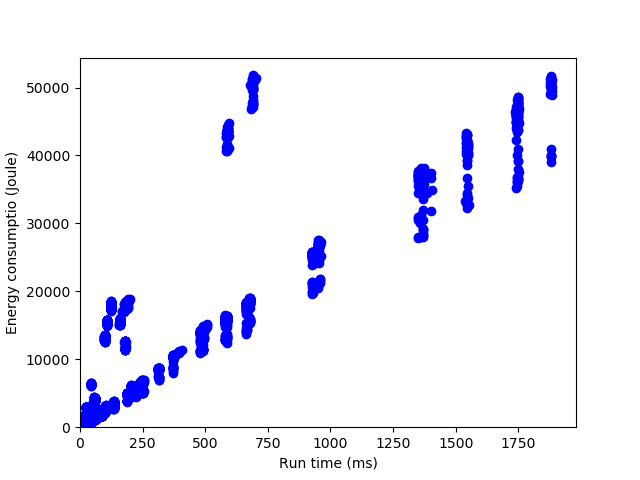
\includegraphics[width=.6\textwidth]{graphs/time.png}
%     \caption{All the measurements from both the measurement nodes, where one dot is one run of a single program.}
%     \label{fig:time}
% \end{figure}

\begin{figure}[h]
    \begin{subfigure}[b]{0.45\textwidth}
        \centering
        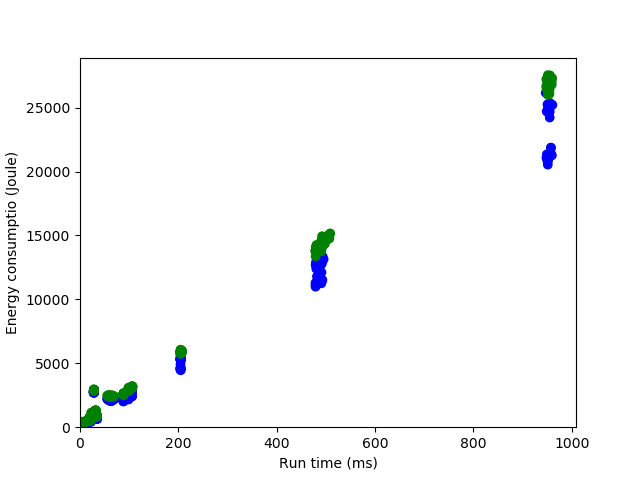
\includegraphics[width=\textwidth]{graphs/time-problem0.png}
        \caption{Binarytrees, tau=0.85}
        \label{fig:time0}
    \end{subfigure}
    \begin{subfigure}[b]{0.45\textwidth}
        \centering
        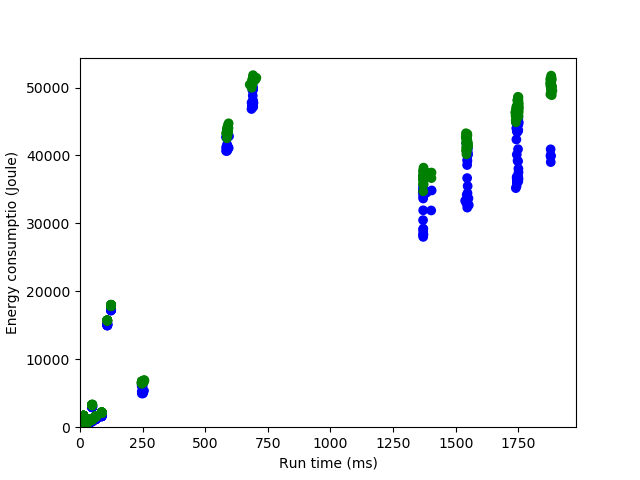
\includegraphics[width=\textwidth]{graphs/time-problem1.png}
        \caption{Fannkuchredux, tau=0.72}
        \label{fig:time1}
    \end{subfigure}
    \begin{subfigure}[b]{0.45\textwidth}
        \centering
        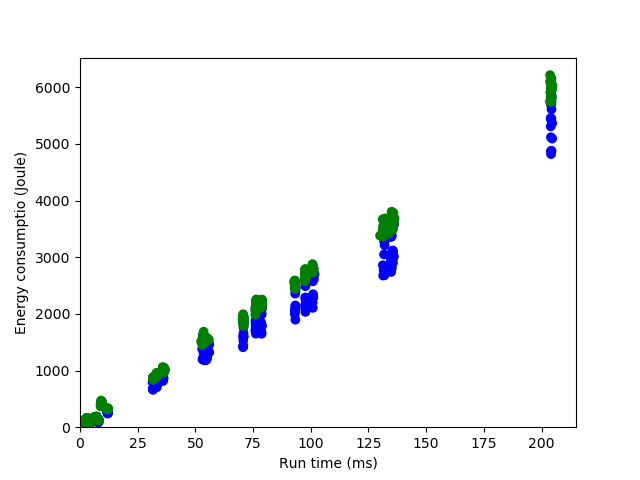
\includegraphics[width=\textwidth]{graphs/time-problem2.png}
        \caption{Fasta, tau=0.84}
        \label{fig:time2}
    \end{subfigure}
    \begin{subfigure}[b]{0.45\textwidth}
        \centering
        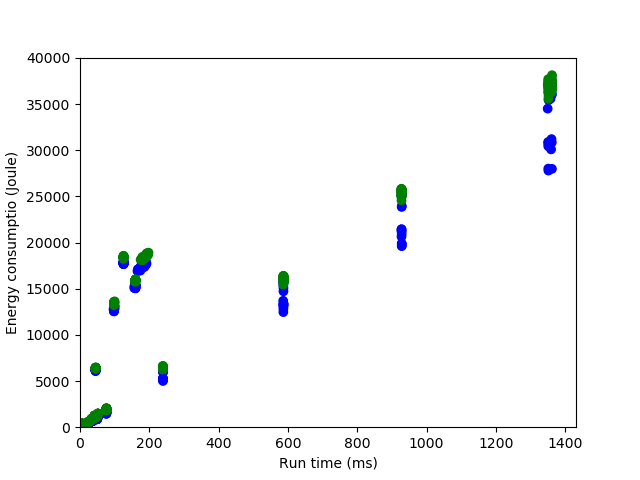
\includegraphics[width=\textwidth]{graphs/time-problem3.png}
        \caption{Mandelbrot, tau=0.84}
        \label{fig:time3}
    \end{subfigure}      
    \begin{subfigure}[b]{0.45\textwidth}
        \centering
        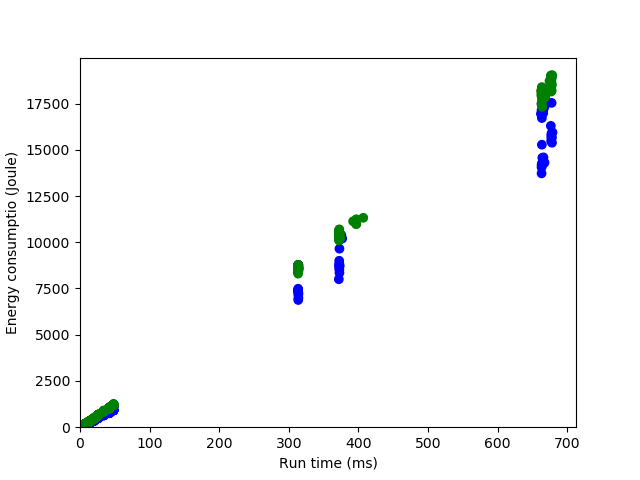
\includegraphics[width=\textwidth]{graphs/time-problem4.png}
        \caption{Nbody, tau=0.89}
        \label{fig:time4}
    \end{subfigure}
    \begin{subfigure}[b]{0.45\textwidth}
        \centering
        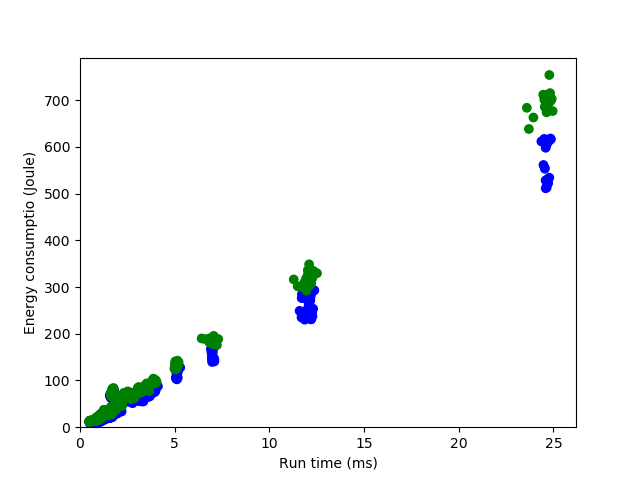
\includegraphics[width=\textwidth]{graphs/time-problem5.png}
        \caption{Revcomp, tau=0.82}
        \label{fig:time5}
    \end{subfigure}
    \begin{subfigure}[b]{0.45\textwidth}
        \centering
        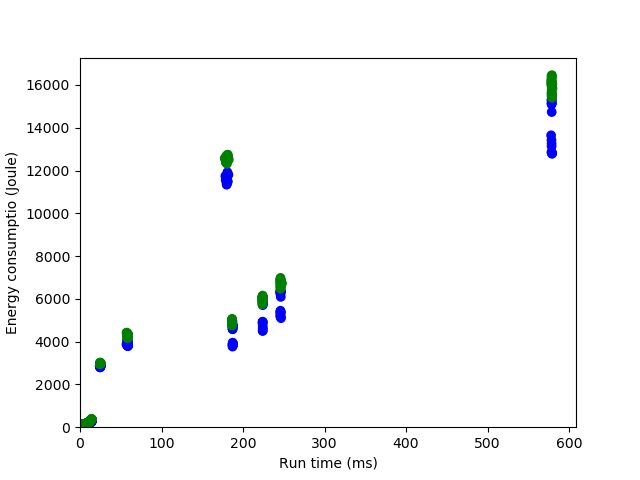
\includegraphics[width=\textwidth]{graphs/time-problem6.png}
        \caption{Spectralnorm, tau=0.85}
        \label{fig:time6}
    \end{subfigure}
    \caption{All the energy measurements and their corresponding run times for every problem. Here the green points are the measurements from \textit{node28} and the blue from \textit{node29}.}
    \label{fig:time}
\end{figure}



